% Options for packages loaded elsewhere
\PassOptionsToPackage{unicode}{hyperref}
\PassOptionsToPackage{hyphens}{url}
%
\documentclass[
]{article}
\usepackage{amsmath,amssymb}
\usepackage{lmodern}
\usepackage{ifxetex,ifluatex}
\ifnum 0\ifxetex 1\fi\ifluatex 1\fi=0 % if pdftex
  \usepackage[T1]{fontenc}
  \usepackage[utf8]{inputenc}
  \usepackage{textcomp} % provide euro and other symbols
\else % if luatex or xetex
  \usepackage{unicode-math}
  \defaultfontfeatures{Scale=MatchLowercase}
  \defaultfontfeatures[\rmfamily]{Ligatures=TeX,Scale=1}
\fi
% Use upquote if available, for straight quotes in verbatim environments
\IfFileExists{upquote.sty}{\usepackage{upquote}}{}
\IfFileExists{microtype.sty}{% use microtype if available
  \usepackage[]{microtype}
  \UseMicrotypeSet[protrusion]{basicmath} % disable protrusion for tt fonts
}{}
\makeatletter
\@ifundefined{KOMAClassName}{% if non-KOMA class
  \IfFileExists{parskip.sty}{%
    \usepackage{parskip}
  }{% else
    \setlength{\parindent}{0pt}
    \setlength{\parskip}{6pt plus 2pt minus 1pt}}
}{% if KOMA class
  \KOMAoptions{parskip=half}}
\makeatother
\usepackage{xcolor}
\IfFileExists{xurl.sty}{\usepackage{xurl}}{} % add URL line breaks if available
\IfFileExists{bookmark.sty}{\usepackage{bookmark}}{\usepackage{hyperref}}
\hypersetup{
  hidelinks,
  pdfcreator={LaTeX via pandoc}}
\urlstyle{same} % disable monospaced font for URLs
\usepackage[margin=1in]{geometry}
\usepackage{longtable,booktabs,array}
\usepackage{calc} % for calculating minipage widths
% Correct order of tables after \paragraph or \subparagraph
\usepackage{etoolbox}
\makeatletter
\patchcmd\longtable{\par}{\if@noskipsec\mbox{}\fi\par}{}{}
\makeatother
% Allow footnotes in longtable head/foot
\IfFileExists{footnotehyper.sty}{\usepackage{footnotehyper}}{\usepackage{footnote}}
\makesavenoteenv{longtable}
\usepackage{graphicx}
\makeatletter
\def\maxwidth{\ifdim\Gin@nat@width>\linewidth\linewidth\else\Gin@nat@width\fi}
\def\maxheight{\ifdim\Gin@nat@height>\textheight\textheight\else\Gin@nat@height\fi}
\makeatother
% Scale images if necessary, so that they will not overflow the page
% margins by default, and it is still possible to overwrite the defaults
% using explicit options in \includegraphics[width, height, ...]{}
\setkeys{Gin}{width=\maxwidth,height=\maxheight,keepaspectratio}
% Set default figure placement to htbp
\makeatletter
\def\fps@figure{htbp}
\makeatother
\setlength{\emergencystretch}{3em} % prevent overfull lines
\providecommand{\tightlist}{%
  \setlength{\itemsep}{0pt}\setlength{\parskip}{0pt}}
\setcounter{secnumdepth}{5}
\usepackage{booktabs}
\usepackage{longtable}
\usepackage{array}
\usepackage{multirow}
\usepackage{wrapfig}
\usepackage{float}
\usepackage{colortbl}
\usepackage{pdflscape}
\usepackage{tabu}
\usepackage{threeparttable}
\usepackage{threeparttablex}
\usepackage[normalem]{ulem}
\usepackage{makecell}
\usepackage{xcolor}
\ifluatex
  \usepackage{selnolig}  % disable illegal ligatures
\fi
\newlength{\cslhangindent}
\setlength{\cslhangindent}{1.5em}
\newlength{\csllabelwidth}
\setlength{\csllabelwidth}{3em}
\newenvironment{CSLReferences}[2] % #1 hanging-ident, #2 entry spacing
 {% don't indent paragraphs
  \setlength{\parindent}{0pt}
  % turn on hanging indent if param 1 is 1
  \ifodd #1 \everypar{\setlength{\hangindent}{\cslhangindent}}\ignorespaces\fi
  % set entry spacing
  \ifnum #2 > 0
  \setlength{\parskip}{#2\baselineskip}
  \fi
 }%
 {}
\usepackage{calc}
\newcommand{\CSLBlock}[1]{#1\hfill\break}
\newcommand{\CSLLeftMargin}[1]{\parbox[t]{\csllabelwidth}{#1}}
\newcommand{\CSLRightInline}[1]{\parbox[t]{\linewidth - \csllabelwidth}{#1}\break}
\newcommand{\CSLIndent}[1]{\hspace{\cslhangindent}#1}

\author{}
\date{\vspace{-2.5em}Manuscript last updated: 16 June, 2021}

\begin{document}

{
\setcounter{tocdepth}{2}
\tableofcontents
}
\hypertarget{front-matter}{%
\section{Front matter}\label{front-matter}}

\textbf{Type of manuscript:}

Original Research Article

~

\textbf{Title: }

Association of lipid-regulating drugs with dementia and related conditions: an observational study of data from the CPRD

~

\textbf{Authors and affiliations:}

Luke A McGuinness\textsuperscript{1,2,*}, Julian PT Higgins\textsuperscript{1,2,3}, Venexia M Walker\textsuperscript{1,2,4}, Neil M Davies\textsuperscript{1,2}, Richard M Martin\textsuperscript{1,2,3}, Elizabeth Coulthard\textsuperscript{5}, George Davey-Smith\textsuperscript{1,2,3}, Patrick G Kehoe\textsuperscript{5,6} and Yoav Ben-Shlomo\textsuperscript{2}

\begin{enumerate}
\def\labelenumi{(\arabic{enumi})}
\tightlist
\item
  MRC University of Bristol Integrative Epidemiology Unit, Bristol, UK
\item
  Bristol Medical School: Population Health Sciences, University of Bristol, Bristol, UK
\item
  NIHR Biomedical Research Centre at University Hospitals Bristol and Weston NHS Foundation Trust and the University of Bristol.
\item
  Department of Surgery, University of Pennsylvania Perelman School of Medicine, Philadelphia, USA
\item
  Bristol Medical School: Translational Health Sciences, University of Bristol, Bristol, UK
\item
  Dementia Research Group, Bristol Medical School, University of Bristol, Bristol, UK
\end{enumerate}

~

\textbf{Corresponding author:}

Luke McGuinness; Bristol Medical School, University of Bristol,
Canynge Hall, 39 Whatley Road, Bristol, BS8 2PS, United Kingdom.; \href{mailto:luke.mcguinness@bristol.ac.uk}{\nolinkurl{luke.mcguinness@bristol.ac.uk}}

~

\textbf{Conflict of interest statement}
None declared.

~

\textbf{Sources of funding}

LAM is supported by an NIHR Doctoral Research Fellowship (DRF-2018-11-ST2-048). JPTH, RMM and GDS are supported by the NIHR Biomedical Research Centre at University Hospitals Bristol and Weston NHS Foundation Trust and the University of Bristol. The views expressed are those of the author(s) and not necessarily those of the NIHR or the Department of Health and Social Care. YBS and JPTH are supported by the NIHR Applied Research Collaboration West (ARC West) at University Hospitals Bristol NHS Foundation Trust. LAM, VMW, NMD, RMM, JPTH and GDS are members of the MRC Integrative Epidemiology Unit at the University of Bristol (MC\_UU\_00011/1). JPTH is a National Institute for Health Research (NIHR) Senior Investigator (NF-SI-0617-10145).
The views expressed in this article are those of the authors and do not necessarily represent those of the NHS, the NIHR, MRC, or the Department of Health and Social Care.

~

\textbf{Word counts}

\begin{itemize}
\tightlist
\item
  Main text word count (max 3000): 3021
\item
  Abstract word count (max 250): 203
\end{itemize}

~

\textbf{Data/code availability}
This analysis used the CPRD-GOLD primary care dataset March 2016 snapshot (ISAC 15\_246R), which is available upon application to the CPRD Independent Scientific Advisory Committee. The code lists used to define the outcomes and covariates for this study, in addition to the cleaning and analysis scripts used to create the study cohort and perform the analyses, are available on GitHub (\url{https://github.com/mcguinlu/CPRD-LRA}), and were archived at the time of submission on Zenodo (DOI: \textbf{TBC}).

\newpage

\hypertarget{abstract}{%
\section{Abstract}\label{abstract}}

\textbf{Background:} There is some evidence that circulating blood lipids play a role in the development of Alzheimer's disease and dementia. As a result, these readily modifiable risk factors could be targeted by existing lipid-regulating agents, including statins, for the prevention of dementia. Here, we assess the association between lipid-regulating agents and subsequent risk of dementia and related conditions in the Clinical Practice Research Datalink (CPRD), a large scale electronic health record database.

\textbf{Methods:} A retrospective cohort study design using data from the CPRD, routinely collected between January 1995 and March 2016, was performed. Cox proportional hazard models, allowing for a time-varying treatment indicator, were used to estimate the association between seven lipid-regulating drug classes and five dementia outcomes (all-cause, vascular and other dementia, and probable and possible Alzheimer's disease).

\textbf{Results:} We analyzed 1,695,683 participants with a median follow-up of 5.8 participant-years. We found little evidence that lipid-regulating agents were associated with risk of Alzheimer's disease (probable AD HR: 0.98, 95\%CI: 0.94-1.01; possible AD HR: 0.97, 95\%CI: 0.93-1.01), but there was evidence of an increased risk of all-cause (HR: 1.17, 95\%CI: 1.14-1.19), vascular (HR: 1.81, 95\%CI: 1.73-1.89) and other dementia (HR: 1.19, 95\%CI: 1.15-1.24). Evidence for an increased risk of the control outcome, ischemic heart disease (\texttt{r}ihd\_text`), indicated the presence of substantial residual confounding.

\textbf{Conclusion:} We found little evidence that lipid-regulating agents had any effect on Alzheimer's disease risk. There was some evidence of an increased the risk of all-cause, vascular and other dementia, likely the result of residual confounding by indication.

\textbf{Keywords:} Dementia; Alzheimer's disease; Lipids; Statins; Cohort study; Observational study; Electronic health records

\newpage

\hypertarget{key-messages}{%
\section{Key messages}\label{key-messages}}

\newpage

\hypertarget{introduction}{%
\section{Introduction}\label{introduction}}

Dementia is a major neurocognitive disorder, the most common types of which are Alzheimer's disease (AD) and vascular dementia (VaD).(1) Despite an increasing number of cases globally and decades of research, there remains much unknown about the pathogenesis and progression of the disease, and, at present, no effective treatment exists to arrest or reverse the cognitive decline associated with the condition.(2) Drug repurposing, the identification of new applications for previously approved drugs, may provide an efficient mechanism to discover effective preventative and therapeutic treatments for dementia.(3,4)

Several cardiovascular factors have been identified as potential risk factors for dementia,(5) and of these, circulating lipid levels represent a promising target for intervention due to the ready availability of lipid-modifying treatments. In this context, determining whether lipid-regulating agents (LRA) could be repurposed for the prevention of dementia and related diseases would be helpful in the development of evidence-based prevention policy. Several existing prospective studies have examined the association of LRA use with dementia.(6--10) However, many of these studies are small, record few outcomes, and have limited follow-up.

The use of electronic health data for epidemiological research has several advantages.(11) As the data are collected through the routine care of a large cohort, they allow for nested prospective studies using sample sizes and time-scales which would be unfeasible using traditional methods. In addition, data are collected for care provision and without a specific research question in mind, providing a holistic picture of a patient and their health experience. This provides vital data on a range of potential confounders which can be incorporated into an analysis.

We therefore aim to examine the association between several major classes of LRA and all-cause dementia, Alzheimer's disease, vascular dementia and other dementia, in the Clinical Practice Research Datalink (CPRD), a large, population-based electronic health record (EHR) database.(12)

\newpage

\hypertarget{methods}{%
\section{Methods}\label{methods}}

\hypertarget{study-design-and-protocol}{%
\subsection{Study design and protocol}\label{study-design-and-protocol}}

We performed a cohort study using data from the CPRD. Our initial sample included all participants registered at a participating practice between 1 January 1995 and 29 February 2016 who had a flag for ``research quality'' data. All events of interest were identified using predetermined code lists, which are available for inspection (see \protect\hyperlink{data-code-avail}{Data/code availability}).

An \emph{a priori} protocol for this study was published, (13) and amendments to this are recorded in Supplementary Materials 1. This study was reported in line with the STROBE Cohort guidelines (Supplementary Table 3).(14)

~

\hypertarget{study-cohort}{%
\subsection{Study Cohort}\label{study-cohort}}

Participants were included in our study cohort if their record contained any of the following index events: a Read code for a diagnosis of hypercholesterolemia or related condition; a Read code for prescription of a LRA (such as statins); a total cholesterol test result of \textgreater4mmol/L; or an low density lipoprotein cholesterol (LDL-c) test result of \textgreater2mmol/L.

These index events allowed us to define a population of participants who were either at risk of hypercholesterolemia, as indicated by the elevated total or LDL-c test results, or had already been diagnosed with it, as indicated by a diagnostic code or related prescription. This approach was employed in an attempt to reduce confounding by indication that we would expect to observe in a general population cohort. Conditioning entry into the study on being either ``at-risk'' or already diagnosed with hypercholesterolemia attempts to mitigate this potential bias.

The index date for a participant was defined as the date where the first relevant code or test result (as detailed above) was recorded on their clinical record. Participants were followed up until the earliest of: an outcome of interest; death; end of follow-up (29 February 2016); or last registration date with their GP practice. Participants were removed from our sample if they were less than 40 years of age, had less than 12 months of ``research quality'' data, were simultaneously prescribed more than one LRA (due to the difficulty of assigning these patients to a single exposure group), or were diagnosed with dementia before or on the date of the index event.

~

\hypertarget{exposures}{%
\subsection{Exposures}\label{exposures}}

We considered seven lipid-regulating drug classes based on groupings in the British National Formulary (BNF)(15), namely: statins, fibrates, bile acid sequestrants, ezetimibe, nicotinic acid groups, ezetimibe and statin (representing one treatment containing both drugs, rather than the two classes being prescribed concurrently), and omega-3 fatty acid groups.

A participant's drug class was assigned based on their first recorded prescription, and any drug switching was ignored in an effort to mimic an intention-to-treat approach. We did however tabulate how often the initial drug class was stopped (defined as last prescription of the primary class being followed by at least six months of observation), added to (defined as a second drug class being prescribed before the last prescription of the initial class), or switched (defined as a second drug class being prescribed after the last prescription of the initial class).

~

\hypertarget{outcomes}{%
\subsection{Outcomes}\label{outcomes}}

We considered five outcomes as part of this analysis: probable Alzheimer's disease, possible Alzheimer's disease, vascular dementia, other dementia, and a composite all-cause dementia outcome. When two or more outcomes were coded in a participant's clinical record, a decision tree was used to differentiate between them (Supplementary Figure 1). The diagnosis date of the outcome was determined by the first record of a relevant code.

~

\hypertarget{covariates}{%
\subsection{Covariates}\label{covariates}}

The analysis was adjusted for a range of baseline covariates including sex, grouped year of entry into the cohort (\textless2000, 2000-2004, 2005-2009, \textgreater2010), Charlson co-morbidity index, Index of Multiple Deprivation (IMD), consultation rate, alcohol (current, former, never), smoking (current, former, never), BMI, baseline total cholesterol, and history of cardiovascular disease, coronary bypass surgery, coronary artery disease, peripheral arterial disease, hypertension, chronic kidney disease, and Type 1 and Type 2 diabetes. All
covariates were determined at index and definitions for each can be found in Supplementary Table 1.

~

\hypertarget{analysis-plan}{%
\subsection{Analysis plan}\label{analysis-plan}}

All analyses were performed in STATA 15. Cox proportional hazard models were used to estimate the hazard ratio and corresponding 95\% confidence intervals, allowing for the potential for clustering by practice. To address the potential for immortal time bias, we employed a time-varying indicator of treatment status to correctly allocate time-at-risk to the exposed and unexposed groups.(16) To observe the effect of adjusting for additional covariates, we compared models adjusted for age only (captured by using the participant's age as the time axis for the model(17--19)) and age and sex to the fully adjusted model. Additional analyses stratified by outcome and drug class were also performed.

In the case of missing data, we used multiple imputation by chained equations (MICE) in STATA to create 20 imputed datasets. All covariates included in the analytic model were also included in the imputation model. The full imputation model is available for inspection (See \protect\hyperlink{data-code-avail}{Data/Code availability} section).

~

\hypertarget{additional-analyses}{%
\subsection{Additional analyses}\label{additional-analyses}}

We performed a number of sensitivity analysis. We stratified the analysis by grouped year of entry to explore the potential for a time period effect. As statins are contraindicated in pregnancy,(20) we ran the models described above but excluding participants below the age of 55. We also further stratified the statin exposure group into lipophilic (Atorvastatin, Lovastatin, Simvastatin, Cerivastatin) and hydrophilic (Pravastatin, Rosuvastatin, Fluvastatin) statins. Finally, we include two control outcomes, using the fully adjusted model to investigate the association between LRA and both back pain (negative control) and ischemic heart disease (postive control).

~

\newpage

\hypertarget{results}{%
\section{Results}\label{results}}

\hypertarget{patient-characteristics}{%
\subsection{Patient characteristics}\label{patient-characteristics}}

A total of participants included in our extract, 1,684,564 met the inclusion criteria (See Supplementary Figure 2 for the attrition flowchart), with a total follow-up of 10800903 patient years at risk. The majority of participants were included in the cohort on the basis of an elevated test result (\texttt{r}index\_event\_text`). The median age at index was 57 years (Inter quartile range (IQR):48-68) and participants were followed up for a median of 5.8 years (IQR:2.7-9.7). During follow-up, an all-cause dementia diagnosis was recorded for 41,830 patients (12,647 probable AD, 9,954 possible AD, 8,466 vascular dementia, 10,763 other dementia; see Supplementary Figure 1). The distribution of baseline characteristics across the drug classes can be seen in Table \ref{tab:cprdCharacteristics-table}.

A substantial majority (98.1\%) of participants prescribed a lipid-regulating agent were prescribed a statin. We excluded the ``Ezetimibe and statins'' and ``Nicotinic acid groups'' classes from subsequent analysis based on the extremely small number of participants in these groups (Table \ref{tab:cprdCharacteristics-table}). The ``Ezetimibe and statins'' treatment group represent those prescribed a treatment containing both ezetimibe and statins, rather than those where the two treats were prescribed concurrently. The stopping, addition and switching of drug classes was common across all exposure groups (Supplementary Table 2).

~

\hypertarget{missing-data}{%
\subsection{Missing data}\label{missing-data}}

Full covariate information was available for 451,897 participants (26.6\%). Five key variables had some missing data: IMD 2010 score, a proxy for socioeconomic position that is measured as twentiles with 1 indicating the least deprived and 20 indicating the most deprived, was missing for 630,439 participants (37.2\%), because it is only recorded for English practices; alcohol status was missing for 272,745 participants (16.1\%); smoking status was missing for 85,267 participants (5\%); BMI, or a calculated BMI from height and weight measurements, was missing for 270,122 participants (15.9\%); baseline total cholesterol was missing for 121,101 participants (7.1\%); and baseline LDL cholesterol was missing for 793,720 participants (46.8\%).

~

\hypertarget{primary-analysis}{%
\subsection{Primary analysis}\label{primary-analysis}}

~

All results described below are from the fully adjusted model. The results of the model adjusted only for age and for age and sex are presented in Supplementary Figure 3. Adjustment for additional covariates beyond age and sex had a limited impact on the observed effect estimates, with the exception of the Probable AD outcome. In this case, adjustment for the full set of covariates attenuated to the null the protective effect observed when adjusting only for age and sex.

~

\textbf{Alzheimer's disease}

As shown in Figure \ref{fig:cprdPrimary}, our results show little evidence of an effect of lipid-regulating agents on probable (HR: 0.98, 95\%CI: 0.94-1.01) and possible (HR: 0.97, 95\%CI: 0.93-1.01) Alzheimer's disease when compared with no treatment, with the exception of fibrates on probable Alzheimer's disease (HR: 1.28, 95\%CI: 1.08-1.52).

~

\textbf{Non-Alzheimer's disease dementias}

In contrast to the findings for Alzheimer's disease outcomes, lipid-regulating agents were associated with an increased risk of a subsequent diagnosis of vascular dementia (HR: 1.81, 95\%CI: 1.73-1.89) or other dementia (HR: 1.19, 95\%CI: 1.15-1.24). Again this effect was driven mainly by the statin subgroup, but there was some evidence that ezetimibe was associated with an increased risk of vascular (HR: 2.33, 95\%CI: 1.11-4.89) and other (HR: 1.88, 95\%CI: 1.01-3.5) dementia.

~

\textbf{All-cause dementia}

For the composite all-cause dementia outcome, we found treatment with a lipid-regulating agent was associated with a slightly increased risk (HR: 1.17, 95\%CI: 1.14-1.19), but the magnitude of the association was not as extreme as that observed for the vascular dementia subgroup. There was also some evidence that fibrates were associated with increased risk of all-cause dementia (HR: 1.28, 95\%CI: 1.08-1.52).

~

\hypertarget{sensitivity-analyses}{%
\subsection{Sensitivity analyses}\label{sensitivity-analyses}}

Removing participants aged 55 and under at index from our analysis had minimal effect on our estimates (Supplementary Figure 4).

For our control outcomes (Supplementary Figure 6), there was some evidence that treatment with a lipid-regulating agent was associated with an increased risk of back pain (HR: 1.04, 95\% CI: 1.03-1.05). However, LRA prescription was also associated with a substantially increased risk of ischemic heart disease (HR: 1.62, 95\% CI: 1.59-1.64), suggesting substantial uncontrolled confounding related to vascular factors.

\newpage

\hypertarget{discussion}{%
\section{Discussion}\label{discussion}}

\hypertarget{main-findings}{%
\subsection{Main findings}\label{main-findings}}

There was little evidence that lipid-regulating agents on probable and possible Alzheimer's when compared with no treatment, but some evidence they were associated with an increased risk of an all-cause dementia, vascular dementia and other dementia diagnosis. The effect observed in each case was driven by the statin subgroup, which included a substantial majority of participants. For the other drug classes, there was limited evidence of an association with any outcome, with two exceptions. Ezetimibe was associated with increased risk of vascular and other dementia, while fibrates were associated with increased risk of all-cause dementia and probable Alzheimer's disease.

~

\hypertarget{comparison-to-other-literature}{%
\subsection{Comparison to other literature}\label{comparison-to-other-literature}}

Much of the existing literature focuses on the association of statins alone with neurodegenerative outcomes, with other lipid-regulating agents being grouped as ``non-statin cholesterol-lowering drugs.''(8) This echoes the distribution of participants among subgroups in our analysis, with the statin subgroup including almost all participants.

~

\textbf{Statins and all-cause dementia}

A recent Cochrane Review identified two randomized trials comparing treatment with statins versus non-treatment for the prevention of dementia, only one of which presented information on the incidence of dementia.(21) This study (Heart Protection Study) showed no effect of treatment with simvastatin on all-cause dementia risk (OR: 1.00, 95\%CI:0.61-1.65),(22) but concerns were raised over the diagnostic criteria used. A meta-analysis of 30 observational studies found a reduced risk of all-cause dementia was associated with statin treatment (RR 0.83, 95\%CI: 0.79--0.87).(23)

These sources of evidence conflict with the findings of our analysis, where statin use was associated with an increased risk of all-cause dementia (HR: 1.17, 95\%CI: 1.14-1.19). However, some of the included studies in the meta-analysis specifically exclude vascular dementia from the definition of all-cause dementia,(24) which may lead to an artificial protective effect of statins on all-cause dementia

~

\textbf{Statins and Alzheimer's disease}

Our results are broadly in line with the findings of two distinct approaches examining the effect of statin treatment on subsequent Alzheimer's disease. No randomized trials of statins for the prevention of Alzheimer's disease have been reported, but a recent meta-analysis of 20 observational studies found statins were associated with a reduced risk of Alzheimer's disease (RR 0.69, 95\% CI 0.60--0.80), though the reduction was more extreme than observed in our analysis.(23) In addition, a recent Mendelian randomization study examining the effect of genetic inhibition of HMGCR on Alzheimer's disease found a small reduction in risk of Alzheimer's disease, comparable in magnitude to our findings (OR: 0.91, 95\%CI: 0.63-1.31).(25)

An additional analysis found no difference in effect between lipophilic and hydrophilic statins for the prevention of Alzheimer's disease, consistent with a recent meta-analysis.(6)

~

\textbf{Statins and non-Alzheimer's disease dementia}

Much less literature is available on the association between lipid-regulating agents and vascular dementia or other dementia. A recent review found four observational studies examining the association of statins and vascular dementia found limited evidence for an effect (RR:0.93, 95\% CI 0.74--1.16).(23) This contrasts with the increased effect found in our analysis (HR: 1.81, 95\%CI: 1.73-1.89). An additional analysis found that lipophilic statins were more harmful than hydrophilic statins in vascular dementia, potentially due to their ability to cross the blood brain barrier.

~

\textbf{Other drug classes}

Apart from statins, few studies examining a lipid-regulating agent have been reported. One of the few classes for which data was available were fibrates, for miminal evidence of an effect on all-cause dementia was identified, (8) inconsistent with our finding of a small increase in all-cause dementia risk in those prescribed a fibrate.

To our knowledge, there is no previous study of the effect of preventative treatment with ezetimibe on any dementia outcome, and so we cannot compare our unexpected finding that treatment with the drug associated with an increased risk of the vascular and other dementia outcomes.

~

\hypertarget{strengths-and-limitations}{%
\subsection{Strengths and Limitations}\label{strengths-and-limitations}}

A major strength of our analysis is the size of the included cohort and the length of follow-up that the use of electronic health records allowed. In addition, we followed users and non-users from a common index date, using a time-updating treatment indicator to correctly assign time-at-risk to the exposed and unexposed groups.

However, the findings of our analysis are subject to several limitations. There is a strong possibility of differential misclassification of dementia-related condition based on the exposure, as those with memory complaints are more likely to be classified as vascular dementia than Alzheimer's disease if their medical records contains prescriptions for lipid-regulating agents. Further, there is a potential for non-differential misclassification of the outcome based on the use of electronic health records to identify dementia cases.(26,27)

Our study may be subject to confounding by indication, which occurs when factors that affect whether a participant is exposed also affect their outcome. We attempted to address this by limiting inclusion to those either prescribed or ``at risk'' of being prescribed, which was determined using an elevated test result. We also adjusted for several additional potential confounding variables. However, the negative control analysis of back pain demonstrated a harmful association with lipid-regulating agent use, indicating that our findings may be biased by residual confounding. Important confounding variables for which we have not adjusted could include genetic factors. A recent preprint of a study in the UK Biobank demonstrated that an Alzheimer's disease polygenic risk score was associated with an increased risk of unspecified Alzheimer's and vascular dementia, and also with an increased frequency of self-reported raised cholesterol levels, a diagnosis of hypercholesterolaemia, and a history of taking lipid-regulating agents such as statins or ezetimibe.(28) This finding, combined with the potential for differential misclassification between Alzheimer's disease and vascular dementia, could explain part of the observed association between lipid-regulating agents and vascular dementia.

Finally, there is also the potential for reverse causation in this analysis. Dementia and associated conditions have a long prodromal period, during which preclinical disease could cause indications for the prescription of a lipid-regulating agent.

\newpage

\hypertarget{conclusion}{%
\section{Conclusions}\label{conclusion}}

We have provided new evidence on the potential repurposing of lipid-regulating agents for the prevention of all-cause dementia, Alzheimer's disease, vascular dementia, and other dementia. We found limited evidence to support the use of lipid-regulating agents for the prevention of probable or possible Alzheimer's disease, but were associated with an increased risk of all-cause, vascular and other dementias. In all cases, the estimated associations were driven by those observed in the statin subgroup, which comprised the majority of participants in our cohort.

We have attempted to account for important sources of bias in our analysis and provide a comparison with other available literature. However, there is a strong potential for unmeasured confounding, misclassification and reverse causation, which may relate to the unexpected increase in risk of vascular dementia associated with statin use. Future research should aim to address these potential biases and, while it may be costly in terms of time and resources, a large scale, long-term randomized controlled trial would provide useful additional information on the effect of lipid-regulating agents on the risk of dementia and related outcomes.

\newpage

~



\begin{table}[H]

\caption[(ref:cprdCharacteristics-scaption)]{\label{tab:cprdCharacteristics-table}Patient characteristics by drug class. Summary statistics are presented as ``\% (N)'' unless otherwise specified in the variable name.}
\centering
\fontsize{5}{7}\selectfont
\begin{threeparttable}
\begin{tabular}[t]{>{\raggedright\arraybackslash}p{10em}>{\centering\arraybackslash}p{6em}>{\centering\arraybackslash}p{6em}>{\centering\arraybackslash}p{6em}>{\centering\arraybackslash}p{6em}>{\centering\arraybackslash}p{6em}>{\centering\arraybackslash}p{6em}>{\centering\arraybackslash}p{6em}>{\centering\arraybackslash}p{6em}>{\centering\arraybackslash}p{6em}}
\toprule
\textbf{ } & \textbf{Whole Sample} & \textbf{None} & \textbf{Statins} & \textbf{Bile acid sequestrants} & \textbf{Ezetimibe} & \textbf{Ezetimibe \& Statins} & \textbf{Fibrates} & \textbf{Nicotinic acid groups} & \textbf{Omega-3 Fatty Acid Groups}\\
\midrule
\textbf{Sample size (N)} & 1695683 & 1095857 & 588455 & 5417 & 766 & 127 & 3896 & 168 & 997\\
\midrule
\textbf{Index year \newline(median)} & 2006 & 2007 & 2004 & 2005 & 2004 & 2005 & 2001 & 2001 & 2005\\
\midrule
\textbf{Female} & 53.1\% (900847) & 56.3\% (616801) & 47.2\% (277841) & 66.4\% (3598) & 54.6\% (418) & 52.8\% (67) & 38.6\% (1505) & 54.8\% (92) & 52.7\% (525)\\
\midrule
\textbf{Age} & 57 & 54 & 62 & 57 & 60 & 57 & 58 & 62 & 56\\
\midrule
\textbf{CAD} & 0.4\% (7180) & 0.1\% (614) & 1.1\% (6487) & 0.1\% (6) & 0.9\% (7) & 0.0\% (0) & 1.4\% (53) & 0.0\% (0) & 1.3\% (13)\\
\midrule
\addlinespace
\textbf{CBS} & 0.3\% (5739) & 0.1\% (701) & 0.8\% (4947) & 0.1\% (4) & 0.4\% (3) & 0.0\% (0) & 2.0\% (78) & 0.0\% (0) & 0.6\% (6)\\
\midrule
\textbf{CVD} & 2.2\% (36680) & 1.2\% (12803) & 4.0\% (23567) & 1.7\% (90) & 2.6\% (20) & 2.4\% (3) & 4.4\% (171) & 4.8\% (8) & 1.8\% (18)\\
\midrule
\textbf{Charlson (ever > 0)} & 31.0\% (525566) & 25.5\% (279520) & 40.9\% (240925) & 42.6\% (2308) & 41.8\% (320) & 24.4\% (31) & 50.9\% (1983) & 44.6\% (75) & 40.5\% (404)\\
\midrule
\textbf{IMD-2010 (median)} & 9 & 8 & 9 & 8 & 9 & 13 & 10 & 11 & 10\\
\midrule
\textbf{Consulation rate (mean/SD)} & 5.4 (5.5) & 5.0 (5.0) & 6.3 (6.1) & 8.6 (7.4) & 7.4 (6.6) & 4.8 (4.3) & 7.1 (6.2) & 9.3 (7.7) & 8.0 (8.0)\\
\midrule
\addlinespace
\textbf{Alcohol (ever)} & 85.8\% (1455443) & 86.5\% (947716) & 84.7\% (498304) & 82.8\% (4487) & 83.9\% (643) & 87.4\% (111) & 82.8\% (3226) & 82.7\% (139) & 81.9\% (817)\\
\midrule
\textbf{Smoking (ever)} & 51.1\% (866207) & 47.0\% (515192) & 58.5\% (344540) & 55.2\% (2990) & 57.4\% (440) & 60.6\% (77) & 60.1\% (2342) & 53.6\% (90) & 53.8\% (536)\\
\midrule
\textbf{BMI (mean/SD)} & 27.0 (5.3) & 26.7 (5.2) & 27.7 (5.3) & 26.8 (5.8) & 28.1 (5.7) & 28.1 (4.9) & 29.0 (5.2) & 26.4 (5.0) & 26.8 (5.5)\\
\midrule
\textbf{PAD} & 0.8\% (12879) & 0.4\% (4204) & 1.4\% (8524) & 0.9\% (47) & 0.9\% (7) & 0.8\% (1) & 1.9\% (75) & 6.5\% (11) & 1.0\% (10)\\
\midrule
\textbf{Hypertension} & 16.1\% (273011) & 11.6\% (126891) & 24.5\% (144010) & 12.9\% (697) & 23.9\% (183) & 25.2\% (32) & 25.8\% (1006) & 21.4\% (36) & 15.6\% (156)\\
\midrule
\addlinespace
\textbf{Total cholesterol (mean/SD)} & 5.7 (12.4) & 5.5 (10.8) & 6.2 (15.3) & 5.3 (1.3) & 7.1 (26.5) & 6.7 (1.5) & 6.4 (5.6) & 5.4 (1.5) & 5.6 (1.7)\\
\midrule
\textbf{LDL cholesterol (mean/SD)} & 3.6 (4.8) & 3.4 (5.2) & 4.0 (3.6) & 3.1 (1.0) & 3.9 (1.1) & 4.2 (1.0) & 3.3 (1.8) & 3.4 (0.9) & 3.2 (1.0)\\
\midrule
\textbf{CKD} & 0.1\% (1391) & 0.1\% (814) & 0.1\% (566) & 0.1\% (7) & 0.1\% (1) & 0.0\% (0) & 0.0\% (0) & 0.0\% (0) & 0.3\% (3)\\
\midrule
\textbf{Type 1 Diabetes} & 0.2\% (4057) & 0.1\% (795) & 0.5\% (3206) & 0.3\% (14) & 1.0\% (8) & 0.8\% (1) & 0.8\% (31) & 0.6\% (1) & 0.1\% (1)\\
\midrule
\textbf{Type 2 Diabetes} & 2.9\% (49381) & 1.1\% (12376) & 6.1\% (36182) & 2.3\% (124) & 5.4\% (41) & 4.7\% (6) & 15.8\% (617) & 4.2\% (7) & 2.8\% (28)\\
\bottomrule
\end{tabular}
\begin{tablenotes}
\item \textit{Abbreviations:} 
\item LRA - Lipid regulating agent; IMD - Index of Multiple Deprivation; BMI - Body Mass Index; CAD - Coronary Arterial Disease; CBS - Coronary Bypass Surgery; CVD - Cardiovascular disease; PAD - Peripheral arterial disease; CKD - Chronic Kidney Disease; SD - Standard deviation.
\end{tablenotes}
\end{threeparttable}
\end{table}

~

\begin{figure}
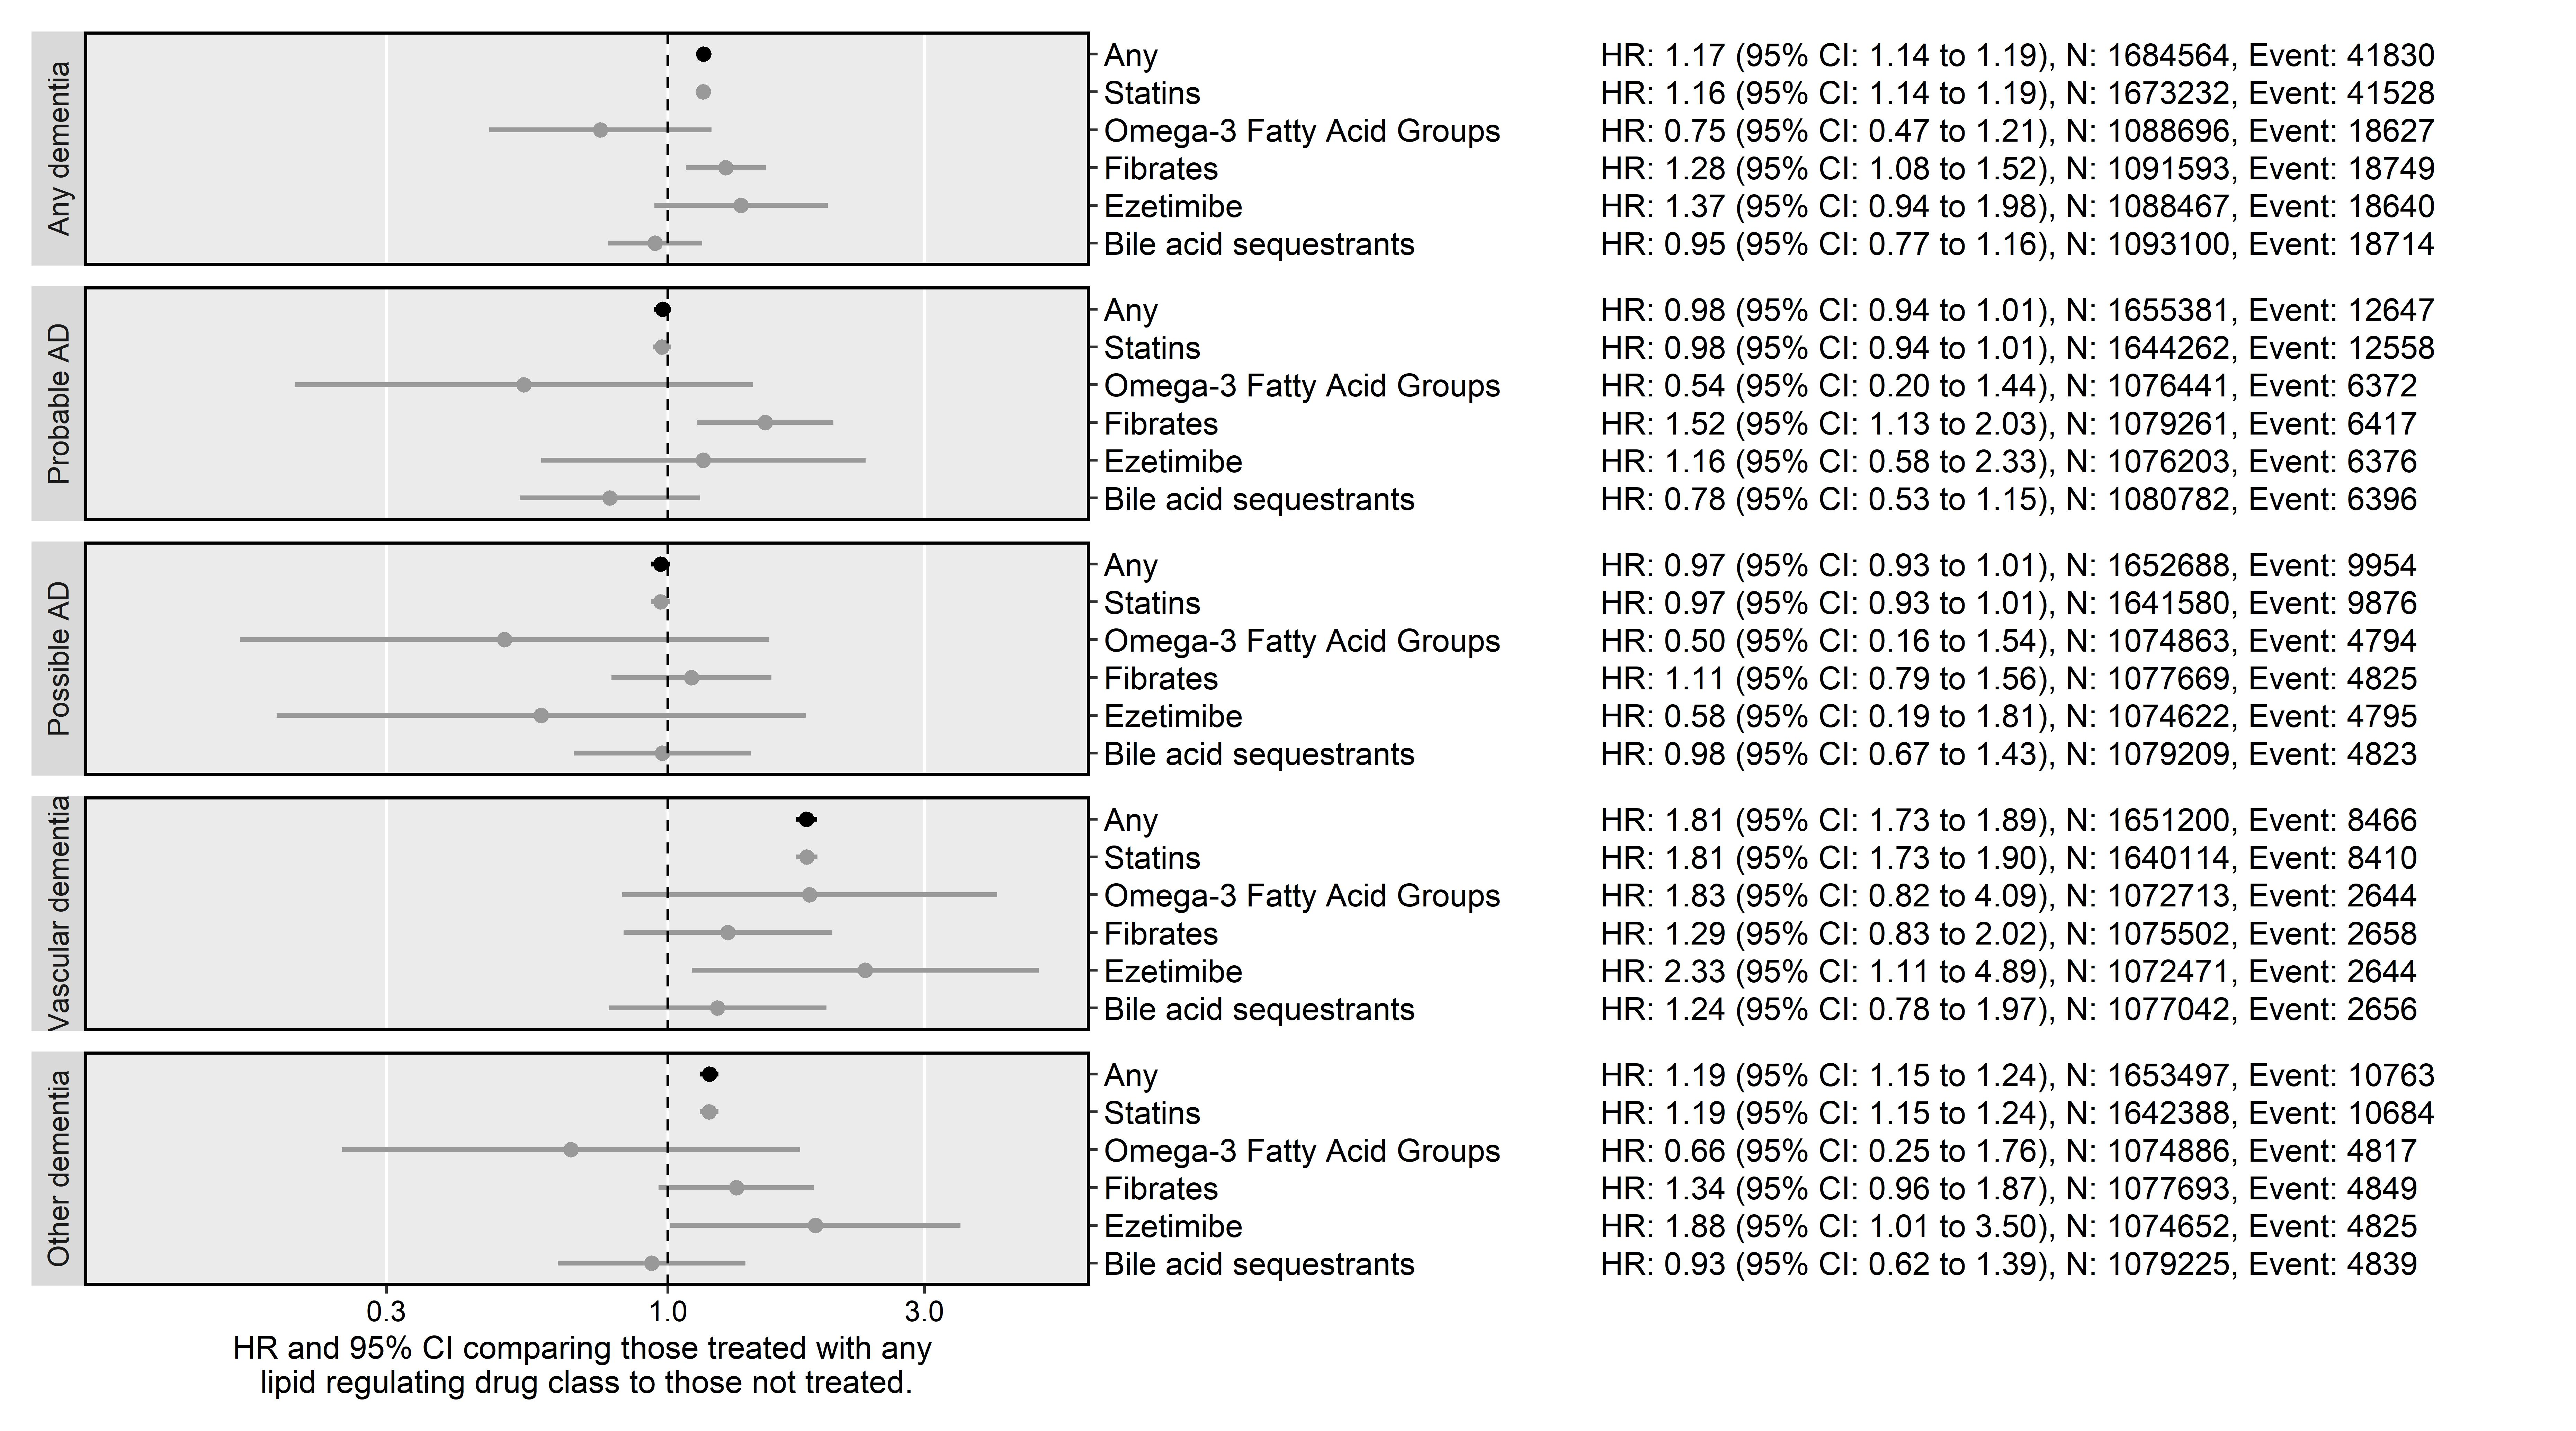
\includegraphics[width=103.33in]{C:/Users/lm16564/OneDrive - University of Bristol/Documents/rrr/thesis/figures/cprd-analysis/fp_p1} \caption{Results from primary analyses of CPRD data using the fully adjusted model and participant age as the time scale.}\label{fig:cprdPrimary}
\end{figure}

\newpage

\hypertarget{bibliography}{%
\section*{Bibliography}\label{bibliography}}
\addcontentsline{toc}{section}{Bibliography}

\hypertarget{refs}{}
\begin{CSLReferences}{0}{0}
\leavevmode\hypertarget{ref-prince2016}{}%
\CSLLeftMargin{1. }
\CSLRightInline{Prince M, Ali G-C, Guerchet M, Prina AM, Albanese E, Wu Y-T. Recent global trends in the prevalence and incidence of dementia, and survival with dementia. Alzheimer's Research \& Therapy. 2016 Jul;8. }

\leavevmode\hypertarget{ref-jobke2018}{}%
\CSLLeftMargin{2. }
\CSLRightInline{Jobke B, McBride T, Nevin L, Peiperl L, Ross A, Stone C, et al. Setbacks in {Alzheimer} research demand new strategies, not surrender. PLoS medicine. 2018 Feb;15(2):e1002518. }

\leavevmode\hypertarget{ref-ashburn2004}{}%
\CSLLeftMargin{3. }
\CSLRightInline{Ashburn TT, Thor KB. Drug repositioning: Identifying and developing new uses for existing drugs. Nature Reviews Drug Discovery. 2004;3(8):673. }

\leavevmode\hypertarget{ref-pushpakom2019}{}%
\CSLLeftMargin{4. }
\CSLRightInline{Pushpakom S, Iorio F, Eyers PA, Escott KJ, Hopper S, Wells A, et al. Drug repurposing: Progress, challenges and recommendations. Nature Reviews Drug Discovery. 2019;18(1):41. }

\leavevmode\hypertarget{ref-walker2019a}{}%
\CSLLeftMargin{5. }
\CSLRightInline{Walker VM, Davies NM, Martin RM, Kehoe PG. Comparison of antihypertensive drug classes for dementia prevention. bioRxiv. 2019 Jan;517482. }

\leavevmode\hypertarget{ref-chu2018}{}%
\CSLLeftMargin{6. }
\CSLRightInline{Chu C-S, Tseng P-T, Stubbs B, Chen T-Y, Tang C-H, Li D-J, et al. Use of statins and the risk of dementia and mild cognitive impairment: {A} systematic review and meta-analysis. Scientific Reports. 2018 Apr;8(1):5804. }

\leavevmode\hypertarget{ref-larsson2018}{}%
\CSLLeftMargin{7. }
\CSLRightInline{Larsson SC, Markus HS. Does {Treating Vascular Risk Factors Prevent Dementia} and {Alzheimer}'s {Disease}? {A Systematic Review} and {Meta}-{Analysis}. Journal of Alzheimer's Disease. 2018 Jan;64(2):657--68. }

\leavevmode\hypertarget{ref-ancelin2012}{}%
\CSLLeftMargin{8. }
\CSLRightInline{Ancelin M-L, Carrière I, Barberger-Gateau P, Auriacombe S, Rouaud O, Fourlanos S, et al. Lipid lowering agents, cognitive decline, and dementia: The three-city study. Journal of Alzheimer's Disease. 2012 Jan;30(3):629--37. }

\leavevmode\hypertarget{ref-bettermann2012}{}%
\CSLLeftMargin{9. }
\CSLRightInline{Bettermann K, Arnold AM, Williamson J, Rapp S, Sink K, Toole JF, et al. Statins, {Risk} of {Dementia}, and {Cognitive Function}: {Secondary Analysis} of the {Ginkgo Evaluation} of {Memory Study}. Journal of Stroke and Cerebrovascular Diseases. 2012 Aug;21(6):436--44. }

\leavevmode\hypertarget{ref-rea2005}{}%
\CSLLeftMargin{10. }
\CSLRightInline{Rea TD, Breitner JC, Psaty BM, Fitzpatrick AL, Lopez OL, Newman AB, et al. Statin {Use} and the {Risk} of {Incident Dementia}: {The Cardiovascular Health Study}. Archives of Neurology. 2005 Jul;62(7):1047--51. }

\leavevmode\hypertarget{ref-casey2016}{}%
\CSLLeftMargin{11. }
\CSLRightInline{Casey JA, Schwartz BS, Stewart WF, Adler NE. Using {Electronic Health Records} for {Population Health Research}: {A Review} of {Methods} and {Applications}. Annual Review of Public Health. 2016 Mar;37(1):61--81. }

\leavevmode\hypertarget{ref-herrett2015}{}%
\CSLLeftMargin{12. }
\CSLRightInline{Herrett E, Gallagher AM, Bhaskaran K, Forbes H, Mathur R, van Staa T, et al. Data {Resource Profile}: {Clinical Practice Research Datalink} ({CPRD}). International Journal of Epidemiology. 2015 Jun;44(3):827--36. }

\leavevmode\hypertarget{ref-walker2016a}{}%
\CSLLeftMargin{13. }
\CSLRightInline{Walker VM, Davies NM, Jones T, Kehoe PG, Martin RM. Can commonly prescribed drugs be repurposed for the prevention or treatment of {Alzheimers} and other neurodegenerative diseases? {Protocol} for an observational cohort study in the {UK Clinical Practice Research Datalink}. BMJ Open. 2016;6(12). }

\leavevmode\hypertarget{ref-vonelm2008}{}%
\CSLLeftMargin{14. }
\CSLRightInline{von Elm E, Altman DG, Egger M, Pocock SJ, Gøtzsche PC, Vandenbroucke JP. The {Strengthening} the {Reporting} of {Observational Studies} in {Epidemiology} ({STROBE}) statement: Guidelines for reporting observational studies. Journal of Clinical Epidemiology. 2008 Apr;61(4):344--9. }

\leavevmode\hypertarget{ref-wishart2017}{}%
\CSLLeftMargin{15. }
\CSLRightInline{Wishart DS, Feunang YD, Guo AC, Lo EJ, Marcu A, Grant JR, et al. {DrugBank} 5.0: A major update to the {DrugBank} database for 2018. Nucleic Acids Research. 2017;46(D1):D1074--82. }

\leavevmode\hypertarget{ref-levesque2010}{}%
\CSLLeftMargin{16. }
\CSLRightInline{Lévesque LE, Hanley JA, Kezouh A, Suissa S. Problem of immortal time bias in cohort studies: Example using statins for preventing progression of diabetes. BMJ. 2010 Mar;340. }

\leavevmode\hypertarget{ref-lamarca1998}{}%
\CSLLeftMargin{17. }
\CSLRightInline{Lamarca R, Alonso J, Gomez G, Munoz A. Left-truncated {Data With Age} as {Time Scale}: {An Alternative} for {Survival Analysis} in the {Elderly Population}. The Journals of Gerontology Series A: Biological Sciences and Medical Sciences. 1998 Sep;53A(5):M337--43. }

\leavevmode\hypertarget{ref-gail2009}{}%
\CSLLeftMargin{18. }
\CSLRightInline{Gail MH, Graubard B, Williamson DF, Flegal KM. Comments on {`{Choice} of time scale and its effect on significance of predictors in longitudinal studies'} by {Michael J}. {Pencina}, {Martin G}. {Larson} and {Ralph B}. {D}'{Agostino}, {\emph{Statistics}}{ \emph{in} }{\emph{Medicine}} 2007; {\textbf{26}} :1343-1359. Statistics in Medicine. 2009 Apr;28(8):1315--7. }

\leavevmode\hypertarget{ref-pencina2007}{}%
\CSLLeftMargin{19. }
\CSLRightInline{Pencina MJ, Larson MG, D'Agostino RB. Choice of time scale and its effect on significance of predictors in longitudinal studies. Statistics in Medicine. 2007 Mar;26(6):1343--59. }

\leavevmode\hypertarget{ref-nationalinstituteforhealthandcareexcellence}{}%
\CSLLeftMargin{20. }
\CSLRightInline{National Institute for Health and Care Excellence. Cardiovascular disease: Risk assessment and reduction, including lipid modification. https://www.nice.org.uk/guidance/cg181/ifp/chapter/Drug-treatments-to-lower-your-cholesterol; {NICE}; }

\leavevmode\hypertarget{ref-mcguinness2016a}{}%
\CSLLeftMargin{21. }
\CSLRightInline{McGuinness B, Craig D, Bullock R, Passmore P. Statins for the prevention of dementia. Cochrane Database of Systematic Reviews. 2016;(1). }

\leavevmode\hypertarget{ref-heartprotectionstudycollaborativegroup2002}{}%
\CSLLeftMargin{22. }
\CSLRightInline{Heart Protection Study Collaborative Group. {MRC}/{BHF Heart Protection Study} of cholesterol lowering with simvastatin in 20 536 high-risk individuals: A randomised placebocontrolled trial. The Lancet. 2002 Jul;360(9326):7--22. }

\leavevmode\hypertarget{ref-poly2020}{}%
\CSLLeftMargin{23. }
\CSLRightInline{Poly TN, Islam MM, Walther BA, Yang H-C, Wu C-C, Lin M-C, et al. Association between {Use} of {Statin} and {Risk} of {Dementia}: {A Meta}-{Analysis} of {Observational Studies}. Neuroepidemiology. 2020;54(3):214--26. }

\leavevmode\hypertarget{ref-chao2015}{}%
\CSLLeftMargin{24. }
\CSLRightInline{Chao T-F, Liu C-J, Chen S-J, Wang K-L, Lin Y-J, Chang S-L, et al. Statins and the risk of dementia in patients with atrial fibrillation: {A} nationwide population-based cohort study. International Journal of Cardiology. 2015 Oct;196:91--7. }

\leavevmode\hypertarget{ref-williams}{}%
\CSLLeftMargin{25. }
\CSLRightInline{Williams DM, Finan C, Schmidt AF, Burgess S, Hingorani AD. Lipid lowering and {Alzheimer}'s disease risk: A {Mendelian} randomization study. Annals of Neurology. 2019;n/a(n/a). }

\leavevmode\hypertarget{ref-wilkinson2018}{}%
\CSLLeftMargin{26. }
\CSLRightInline{Wilkinson T, Ly A, Schnier C, Rannikmäe K, Bush K, Brayne C, et al. Identifying dementia cases with routinely collected health data: {A}~systematic review. Alzheimer's \& Dementia. 2018 Aug;14(8):1038--51. }

\leavevmode\hypertarget{ref-mcguinness2019b}{}%
\CSLLeftMargin{27. }
\CSLRightInline{McGuinness LA, Warren-Gash C, Moorhouse LR, Thomas SL. The validity of dementia diagnoses in routinely collected electronic health records in the {United Kingdom}: {A} systematic review. Pharmacoepidemiology and Drug Safety. 2019 Feb;28(2):244--55. }

\leavevmode\hypertarget{ref-korologou-linden2020}{}%
\CSLLeftMargin{28. }
\CSLRightInline{Korologou-Linden R, Anderson EL, Howe LD, Millard LAC, Ben-Shlomo Y, Williams DM, et al. The causes and consequences of {Alzheimer}'s disease: Phenome-wide evidence from {Mendelian} randomization. medRxiv. 2020 Mar;2019.12.18.19013847. }

\end{CSLReferences}

\end{document}
